
\section{Выбор хранилища данных}

\indent Система планирования производства, как и практически любая система получающая и обрабатывающая данные, нуждается в хранилище данных - базе данных.
Хранилище данных может быть разделено на две составляющие:
\begin{itemize}
	\item хранилище временных данных;
	\item хранилище постоянных данных.
\end{itemize}

\indent Под временными данными подразумеваются данные, которые получаются в процессе работы системы (например оперативные и объемно-календарные планы) и, при необходимости, могут быть рассчитаны заново, хоть и с некоторыми затратами (время, вычислительные мощности), при условии отсутствия хранилища данных.
В данной работе этот вид данных и хранилище для них не рассматривается.\\
\indent С другой стороны постоянные данные - данные, которые задаются пользователем (в данном случае организацией) и потеря которых в лучшем случае приведет к необходимости заново добавлять их в систему, а в худшем - приведет к утрате этих данных.
В любом случае потеря постоянных данных ведет к нарушениям в работе системы, что ведет к необходимости организации консистентного хранилища данных.\\
\indent Консистентность - требование к данным, получаемым из базы данных, которое заключается в том, что последние должны быть целостны и непротиворечивы.
Под целостностью данных подразумевается соответствие имеющейся в базе данных информации её внутренней логике, структуре и явно заданным правилам.
Любое правило, направленное на ограничение возможного состояния базы данных называют ограничением целостности.
Помимо целостных, данные должны также быть непротиворечивыми, что означает, что в базе данных нет логического противоречия, то есть некоторого утверждения и его отрицания.
Со стороны систем управления базами данных (совокупность программных и лингвистических средств общего или специального назначения, обеспечивающих управление созданием и использованием баз данных) свойство консистентности выполняется на уровне транзакций (одним из требований к которой и является консистентность): если одна из команд транзакции не прошла проверку ограничений целостности, то вся транзакция откатывается, то есть база данных возвращается в состояние, в котором была начата транзакция.\\
\indent Транзакция - группа последовательных операций с базой данных, которая представляет собой логическую единицу работы с данными.
Транзакция может либо быть целиком и успешно независимо от идущих параллельно транзакций и соблюдая все ограничения целостности, либо не быть выполненной вообще, что в таком случае не должно оказать на систему никакого влияния.\\
\indent В соответствии с требованиями описанными выше, можно сделать вывод о необходимости использования реляционной базы данных, одним из преимуществ которой является соответствие требованиям ACID (Atomicity, Consistency, Isolation, Durability - атомарность, консистентность, которая и интересует в первую очередь, изолированность, долговечность).

\section{Структура базы данных}

\indent Из предыдущей главы видно, что в постоянной базе данных необходимо хранить информацию по которой будет производиться расчет объемно-календарного и оперативного планов.
Для этого необходимо хранить:

\begin{itemize}
	\item данные о заказах;
	\item данные о типах продукции;
	\item данные о продукции, которая относится к каждому заказу;
	\item данные о самой последовательности операций и самих операциях для каждого типа продукции;
	\item данные о каждой модели ресурсов;
	\item данные о связях между моделью ресурса и операциями.
\end{itemize}

\begin{figure}[ht]	
	\centering	
	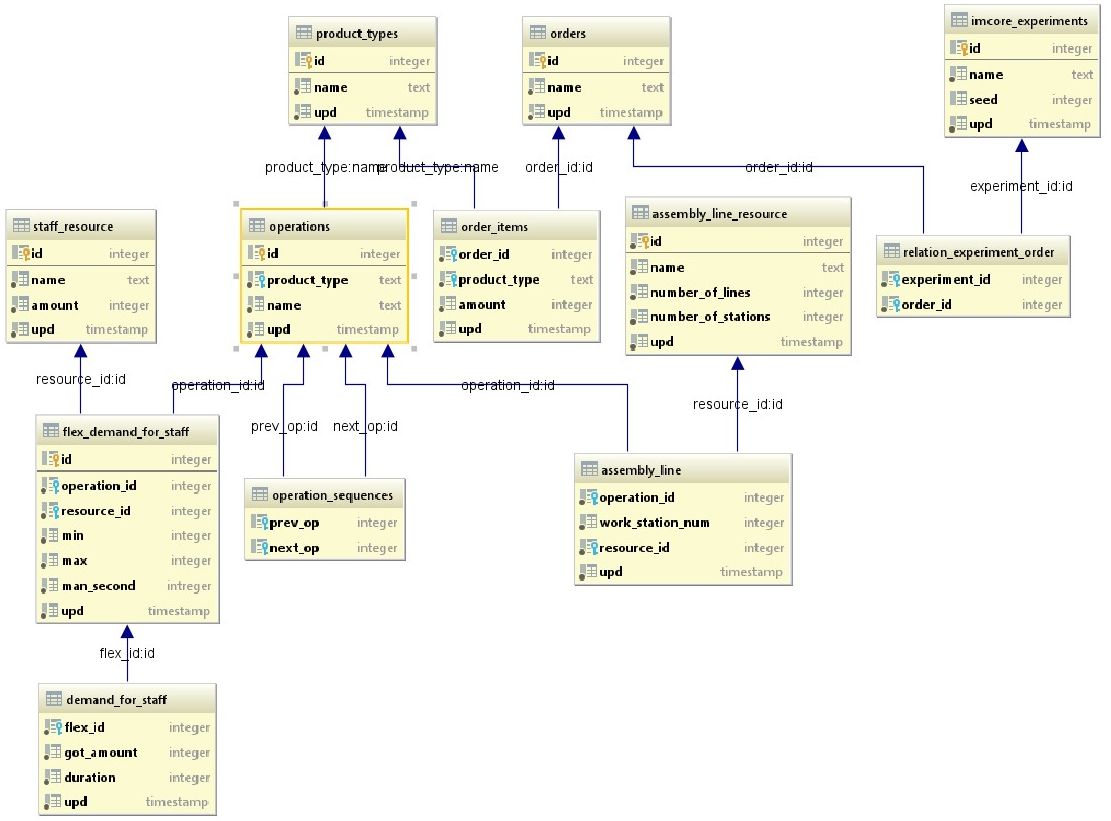
\includegraphics[width=\linewidth]{pics/databaseSchema.png}
	\caption{Схема базы данных}
	\label{fig:dbSchema}
\end{figure}

\indent Помимо этого, нужно учитывать, что кроме простого хранения данных, необходимо соблюдать ``версионность'', ввиду того, что карта технологического процесса может меняться во времени, а значит и в базе данных, требуется следить за тем, чтобы в любой момент времени было возможно использовать любую из версий данной карты, иначе новый расчет оперативного плана (при условии, что другие данные остались неизменными) приведет к созданию новой версии плана, а, следовательно, предыдущую версию восстановить будет либо очень сложно, либо, в худшем случае - невозможно.\\
\indent Для достижения данной цели, в определенных таблицах было введено дополнительное поле - временная отметка обновления - ``upd''.
С помощью этой метки можно как получить последние данные из базы, просто максимизируя метку ``upd'', так и получить данные на определенный момент времени ограничивая эту метку необходимым временем.